\documentclass[11pt]{article}
\usepackage[a4paper,margin=2.3cm]{geometry}
\usepackage{amsmath,amssymb,amsthm,graphicx,booktabs,xcolor}
\usepackage[colorlinks,linkcolor=blue!50!black,urlcolor=blue!50!black,citecolor=blue!50!black]{hyperref}
\newtheorem{theorem}{Theorem}[section]\newtheorem{proposition}[theorem]{Proposition}
\newtheorem{lemma}[theorem]{Lemma}\newtheorem{corollary}[theorem]{Corollary}
\theoremstyle{definition}\newtheorem{definition}[theorem]{Definition}\newtheorem{remark}[theorem]{Remark}\newtheorem{example}[theorem]{Example}
\newcommand{\C}{\mathbb{C}}\newcommand{\R}{\mathbb{R}}\newcommand{\PP}{\mathbb{P}}
\newcommand{\ip}[2]{\langle #1,#2\rangle}\newcommand{\pt}{\mathrm{pt}}\newcommand{\Qd}{\mathcal{Q}}
\newcommand{\chk}[1]{\hfill{\footnotesize\textsf{[#1]}}}
\renewcommand{\Re}{\operatorname{Re}}\renewcommand{\Im}{\operatorname{Im}}
\title{Hidden intersections as a kei of complex circles:\\ mirrors, common points and invariants}
\author{Carlo Perassi}
\date{October 2026\\\small Theory note accompanying a reply to Inigo Quilez's YouTube Short}
\begin{document}\maketitle
\begin{abstract}
A real line that misses a circle still meets it in two complex points. We study this phenomenon inside complex Möbius geometry. Generalized circles are points $[a:b:c:d]$ of $\PP^3(\C)$ with the quadratic form $Q=b^2+c^2-4ad$; reflecting a circle $C$ in a mirror $L$ is the orthogonal reflection $C\star L=C-2\ip CL L/Q(L)$. We prove that $\star$ is a kei (up to the usual projective scale), that its maps generate $PO(4,\C)$, and that a circle meets its mirror image exactly where it meets the mirror: $C\cap L$ equals the finite part of $C\cap(C\star L)$ whenever $\ip CL\neq0$. Common points are counted on the quadric $\{Q=0\}\cong\PP^1\times\PP^1$, where the missing ones live over the circular points. The projective invariant $\kappa=\ip CL^2/(Q(C)Q(L))$ detects tangency ($\kappa=1$), equals $\cos^2$ of the angle for real configurations, and can be negative over $\C$. We describe the real structures that decide which points are visible, compositions of two mirrors (including a complex angle), and the inverse problem of finding the mirror that swaps two circles (exactly two, orthogonal). Every proposition is backed by a symbolic or numerical check.
\end{abstract}
\tableofcontents
\smallskip\noindent\textbf{Roadmap.} §2--3 set up circle space and the mirror; §4 identifies the group; §5--6 prove the common-points theorem and study $\kappa$; §7 explains which points are visible; §8--9 treat two mirrors and the inverse problem; §10 relates all this to Quilez's Short; Appendix~A summarizes phantom loci of general curves.

\section{Introduction}
In the Short \emph{``Intersections are always there''} \cite{IQ}, Inigo Quilez intersects a ray with a circle, keeps the square root when its argument turns negative, and plots real and imaginary parts as the line moves: a line that misses a circle still meets it, at two complex points. This note puts that observation in the setting of complex inversive geometry, where circles, lines, points and ``imaginary circles'' are all vectors in one space and reflecting in a circle is a linear map.

\textbf{Conventions.} We write the mirror on the \emph{right}: $C\star L$ is ``$C$ reflected in $L$''. (The companion note \texttt{alt\_quandle\_note} writes $L\star C$ for the same thing.) All forms are bilinear over $\C$: no complex conjugation appears unless we say so. ``Circle'' means generalized circle (lines included). Worked examples are in the companion \texttt{examples16.pdf}; we cite them as Ex.~1--16.

\textbf{Verification.} Each statement carries a tag such as \textsf{[P3.1]}. The script \texttt{theory\_verify.py} runs the matching exact SymPy checks or numerical tests and writes \texttt{theory\_verify\_log.txt}. Results quoted from earlier notes are checked by \texttt{verify.py}, \texttt{verify\_inversive.py}, \texttt{alt\_verify.py} and \texttt{examples16.py}. Appendix~\ref{app:ver} lists the logs. Numerical checks are evidence, not proofs; every statement also has a written proof or a precise reference.

\section{The space of circles}\label{sec:space}
\begin{definition}
A \emph{(generalized) circle} is a point $C=[a:b:c:d]\in\PP^3(\C)$, read as the curve $a(x^2+y^2)+bx+cy+d=0$ in $\C^2$. It is a \emph{line} if $a=0$. On $\C^4$ put
\[ \ip XY=X^{\mathsf T}GY=bb'+cc'-2(ad'+a'd),\qquad Q(X)=\ip XX=b^2+c^2-4ad,\]\[ G=\begin{pmatrix}0&0&0&-2\\0&1&0&0\\0&0&1&0\\-2&0&0&0\end{pmatrix}. \]
For $p=(x_0,y_0)\in\C^2$ let $\pt(p)=[1:-2x_0:-2y_0:x_0^2+y_0^2]$ (the point-circle at $p$), and $\infty=[0:0:0:1]$.
\end{definition}

\begin{proposition}\label{prop:form}\chk{P2.1}
(a) $G$ is non-degenerate; over $\R$ it has signature $(3,1)$.
(b) For $a\ne0$ the circle has centre $m=(-\tfrac b{2a},-\tfrac c{2a})$ and $r^2=|m|^2-\tfrac da$ (with $|m|^2=m_1^2+m_2^2$, no conjugation), and $Q=4a^2r^2$.
(c) $Q(\pt(p))=0$ and $\ip{\pt(p)}{C}=-2\,C(p)$, where $C(p)$ is the left side of the equation at $p$. So \emph{incidence is orthogonality}: $p\in C\iff\ip{\pt(p)}C=0$.
(d) The null quadric $\Qd=\{Q=0\}\subset\PP^3$ consists of the points $\pt(p)$, $p\in\C^2$ (those with $a\neq0$), together with the \emph{ideal points} $a=0$, $b^2+c^2=0$: the point $\infty$ and the two lines $\{[0:1:i:\delta]\}$, $\{[0:1:-i:\delta]\}$ through it.
\end{proposition}
\begin{proof}
(a) $Q=b^2+c^2+(a-d)^2-(a+d)^2$. (b), (c) are direct expansions. (d) If $a\neq0$, scale to $a=1$; then $d=(b^2+c^2)/4$ is the value that makes $[1:b:c:d]=\pt(-b/2,-c/2)$. If $a=0$ then $Q=b^2+c^2$, which vanishes iff $c=\pm ib$; $b=c=0$ gives $\infty$.
\end{proof}

\begin{proposition}[The quadric is $\PP^1\times\PP^1$]\label{prop:segre}\chk{P2.2}
With $u=x+iy$, $v=x-iy$, the Segre map $([u_0:u_1],[v_0:v_1])\mapsto[u_0v_0:-(u_1v_0+u_0v_1):i(u_1v_0-u_0v_1):u_1v_1]$ is an isomorphism $\PP^1\times\PP^1\to\Qd$ sending $(u,v)=(x+iy,x-iy)$ to $\pt(x,y)$. The ideal points are exactly $u=\infty$ or $v=\infty$, and $\infty=(\infty,\infty)$. In these coordinates a circle is $a\,uv+\tfrac{b-ic}{2}u+\tfrac{b+ic}{2}v+d=0$.
\end{proposition}
\begin{proof}
Nullity and the formulas are direct substitutions (checked symbolically). A smooth quadric surface in $\PP^3(\C)$ is isomorphic to $\PP^1\times\PP^1$ via its two rulings \cite[Ex.~2.21]{Har92}; the displayed map is that isomorphism for our $G$.
\end{proof}

\begin{remark}[Circular points]\label{rem:IJ}\chk{P2.3}
In the projective plane with coordinates $(X:Y:W)$ every circle $a(X^2+Y^2)+bXW+cYW+dW^2$ passes through $I=(1:i:0)$ and $J=(1:-i:0)$, and, if $a\neq0$, its tangent at $I$ is the isotropic line $X+iY+\tfrac{b+ic}{2a}W=0$, i.e.\ the ideal point $[0:1:i:\tfrac{b+ic}{2a}]\in\Qd$, which is orthogonal to $C$. So the ideal points of $\Qd$ on the $I$-line record \emph{tangent directions at $I$} (similarly for $J$). Heuristically, $\Qd$ is $\PP^2$ blown up at $I,J$ with the line at infinity contracted to $\infty$ \cite{Har92}. Two circles meet in $4$ points of $\PP^2$ (Bézout); $I$ and $J$ are always among them, and the other two are what we count on $\Qd$. For two circles with $a\neq0$, an ideal common point on the $I$-line exists exactly when they share their tangent at $I$ (likewise for $J$) (e.g.\ concentric circles, Ex.~5). We only use the checked statements above; the blow-up description is quoted, not proved.
\end{remark}

\section{The mirror operation}\label{sec:star}
\begin{definition}
For $L\in\C^4$ with $Q(L)\neq0$ (a \emph{mirror}) define $s_L(X)=X-\dfrac{2\ip XL}{Q(L)}L$ and $C\star L=s_L(C)$.
\end{definition}

\begin{proposition}[Reflection, closure, involution]\label{prop:refl}\chk{P3.1}
$s_L$ is the orthogonal reflection in the hyperplane $L^\perp$: it fixes $L^\perp$ pointwise, sends $L\mapsto-L$, preserves $\ip{}{}$, and $s_L^2=\mathrm{id}$. It is linear in $X$ and unchanged by $L\mapsto\lambda L$, so $\star$ is well defined on $\PP^3\times\{Q\ne0\}$. Consequently $Q(C\star L)=Q(C)$; the sets $\{Q\neq0\}$ and $\Qd$ are both preserved; and $(C\star L)\star L=C$.
\end{proposition}
\begin{proof}
$\ip{s_LX}{s_LY}=\ip XY-4\ip XL\ip YL/Q(L)+4\ip XL\ip YL Q(L)/Q(L)^2=\ip XY$. The rest is immediate.
\end{proof}

\begin{proposition}[Real mirrors]\label{prop:real}\chk{P3.2}
For a real circle $L$ with centre $m$ and radius $r>0$, $\pt(p)\star L=\pt\big(m+r^2\frac{p-m}{|p-m|^2}\big)$: inversion. For a real line it is the Euclidean reflection. For the imaginary circle $x^2+y^2=-1$ (real coefficients, $Q=-4$) it is $p\mapsto -p/|p|^2$ (Ex.~9).
\end{proposition}
The formula extends these maps to all of $\C^2$, where $|p-m|^2=(p_1-m_1)^2+(p_2-m_2)^2$ is the complex-bilinear square; at its zeros (points on the isotropic lines through $m$) the image is an ideal point.

\begin{theorem}[The circle kei]\label{thm:kei}\chk{T3.3}
On $\mathcal X=\{[C]:Q(C)\neq0\}$, for all $A,B,L$:
\[\text{(K1)}\ L\star L=L,\qquad \text{(K2)}\ (A\star L)\star L=A,\qquad \text{(K3)}\ (A\star B)\star L=(A\star L)\star(B\star L).\]
So $(\mathcal X,\star)$ is a kei (involutory quandle) \cite{Tak43,Joy82,Sta15}; so is its real part. $\star$ is neither commutative nor associative.
\end{theorem}
\begin{proof}
(K1) $s_L(L)=-L$: equality holds \emph{in $\PP^3$ only}; as vectors $L\star L=-L$. (K2) is $s_L^2=\mathrm{id}$. (K3) For any isometry $g$, $g\,s_B\,g^{-1}=s_{gB}$, since $s_{gB}(X)=X-2\ip{X}{gB}gB/Q(B)=g\,s_B(g^{-1}X)$. With $g=s_L$: $s_{B\star L}=s_Ls_Bs_L$, and applying this to $A\star L=s_LA$ gives (K3). Counterexamples to commutativity and associativity: Ex.~7 versus Ex.~2, and Ex.~14.
\end{proof}
\begin{remark}[Domain caveats]\label{rem:dom}
(i) Point-circles and isotropic lines ($Q=0$) are acted on but cannot act: clearing denominators gives $Q(L)X-2\ip XLL\sim L$ for every $X$ (Ex.~10, 11). (ii) If $\ip CL=0$ then $C\star L=C$: orthogonal circles fix each other (Ex.~4). (iii) (K1) and (K3) hold up to scale, which is all that $\PP^3$ sees.
\end{remark}

\section{The group generated by mirrors}\label{sec:group}
\begin{theorem}\label{thm:group}\chk{T4.1}
The maps $s_L$ ($Q(L)\ne0$) generate the orthogonal group $O(4,\C)$ of $\ip{}{}$; on $\PP^3$ this is $PO(4,\C)=O(4,\C)/\{\pm1\}$. The real mirrors with $Q(L)>0$ (real circles and lines) generate a group acting on $\PP^3(\R)$ as $PO(3,1)$, the Möbius group of the sphere.
\end{theorem}
\begin{proof}
By the Cartan--Dieudonné theorem, over a field of characteristic $\ne2$ every isometry of a non-degenerate $n$-dimensional quadratic space is a product of at most $n$ reflections in non-isotropic vectors \cite{Art57}. Applied over $\C$ and over $\R$ this gives $O(4,\C)$ and $O(3,1)$. For the last claim, reflections in vectors with $Q<0$ are not needed projectively: if $Q(N)<0$, pick an orthogonal basis $e_1,e_2,e_3$ of the positive definite $N^\perp$; then $s_{e_1}s_{e_2}s_{e_3}s_N=-\mathrm{id}$, so $s_N\equiv s_{e_1}s_{e_2}s_{e_3}$ on $\PP^3$. The identification with the Möbius group, generated by inversions, is classical \cite{Sch79}.
\end{proof}
\noindent The check \textsf{[T4.1]} decomposes 200 random elements of $O(4,\C)$ into 4 reflections, and confirms $s_N=-s_{e_1}s_{e_2}s_{e_3}$ for $N=x^2+y^2=-1$. On $\Qd\cong\PP^1\times\PP^1$ the identity component $PSO(4,\C)\cong PSL(2,\C)\times PSL(2,\C)$ acts factorwise by Möbius maps of $u$ and $v$, and elements outside it swap the factors (a standard fact we quote, not prove).

\section{Common points}\label{sec:common}
\begin{definition}
The \emph{common points} of independent circles $C,L$ are the points of $\Qd$ orthogonal to both, i.e.\ $\Qd\cap\PP(U)$ with $V=\mathrm{span}(C,L)$, $U=V^\perp$. Their \emph{finite part} is the set of those of the form $\pt(p)$; by Prop.~\ref{prop:form}(c) it is exactly $\{p\in\C^2:C(p)=L(p)=0\}$, which we write $C\cap L$.
\end{definition}

\begin{theorem}[Common points]\label{thm:common}\chk{T5.1}
Let $C,L$ be independent with $Q(L)\neq0$.
\begin{enumerate}
\item If $\ip CL\neq0$, then $\mathrm{span}(C,C\star L)=\mathrm{span}(C,L)$. Hence $C$ and $C\star L$ have the same common points as $C$ and $L$, on all of $\Qd$; in particular $C\cap L$ is the finite part of $C\cap(C\star L)$.
\item If $\ip CL=0$, then $C\star L=C$ and (1) says nothing.
\item $\Qd\cap\PP(U)$ is: two distinct points if $\det\mathrm{Gram}(C,L)=Q(C)Q(L)-\ip CL^2\neq0$; one point (a double point, tangency) if the Gram matrix has rank $1$; all of the line $\PP(U)$ if the Gram matrix vanishes.
\end{enumerate}
\end{theorem}
\begin{proof}
(1) $C\star L=C-kL$ with $k=2\ip CL/Q(L)\neq0$, so $C\wedge(C\star L)=-k\,C\wedge L$. (2) is Remark~\ref{rem:dom}. (3) $U\cap U^\perp=U\cap V=V\cap V^\perp$, so $Q|_U$ and $Q|_V$ have the same rank. $Q|_U$ is a binary quadratic form: of rank $2$ it has two distinct isotropic lines, of rank $1$ it is a square with one double root, and of rank $0$ every vector of $U$ is null.
\end{proof}
\begin{remark}[Counting and exceptions]\label{rem:count}\chk{E5.2}
``Always two'' means two on $\Qd$, with multiplicity. The finite count drops by the number of ideal common points:
\begin{itemize}
\item \emph{Lines} ($a=0$) all pass through $\infty$: two lines meet at $\infty$ and at one finite point (Ex.~6), and parallel lines meet only at $\infty$, doubly ($\kappa=1$).
\item \emph{Concentric circles} share their tangents at $I$ and $J$: the common points are $[0:1:\pm i:0]$, with no finite point (Ex.~5).
\item \emph{Isotropic lines} ($b^2+c^2=0$, $a=0$) have $Q=0$: they are null vectors themselves, they cannot be mirrors, and they meet a circle in at most one finite point (Ex.~10: $y=ix+1$ meets $x^2+y^2=1$ only at $(0,1)$).
\item The rank-$0$ case needs $Q(C)=Q(L)=\ip CL=0$, e.g.\ two point-circles at zero (complex) distance, $\pt(0,0)$ and $\pt(1,i)$, whose whole span is null.
\item \emph{Point-circles} are allowed as $C$ but not as $L$ (Ex.~11).
\end{itemize}
\end{remark}

\section{The invariant \texorpdfstring{$\kappa$}{kappa}}\label{sec:kappa}
\begin{definition} For $Q(C)Q(L)\ne0$ put $\kappa(C,L)=\dfrac{\ip CL^2}{Q(C)\,Q(L)}$. It is symmetric and independent of scaling. \end{definition}
\begin{proposition}\label{prop:kappa}\chk{P6.1}
\begin{enumerate}
\item $\kappa(gC,gL)=\kappa(C,L)$ for every $g\in O(4,\C)$; in particular $\kappa(C\star M,L\star M)=\kappa(C,L)$ and $\kappa(C\star L,L)=\kappa(C,L)$.
\item $C$ and $L$ are tangent (one double common point) iff $\kappa=1$; they are orthogonal iff $\kappa=0$.
\item Real circles with radii $r_1,r_2$ and centre distance $\delta$: $\ip{C_1}{C_2}/\sqrt{Q_1Q_2}=(r_1^2+r_2^2-\delta^2)/(2r_1r_2)$; when they cross at angle $\theta$, $\kappa=\cos^2\theta$. Two real lines at angle $\theta$: $\kappa=\cos^2\theta$. A circle of radius $r$ and a line at distance $\delta$ from its centre: $\kappa=\delta^2/r^2$.
\item For real $C,L$ with $Q(C),Q(L)>0$: $\kappa<1$ gives two real common points, $\kappa=1$ tangency, $\kappa>1$ a conjugate (``hidden'') pair.
\item Over $\C$ every value occurs: $\kappa(x^2+y^2=1,\ y=mx+c)=c^2/(1+m^2)$. Negative values occur, e.g.\ $\kappa=-1$ for $(x-i)^2+y^2=1$ and $x=0$ (Ex.~8), and $\kappa=-\tfrac14$ for a real circle and the imaginary circle $x^2+y^2=-1$ (Ex.~9). For real $C,L$, $\kappa<0$ forces $Q(C)Q(L)<0$.
\end{enumerate}
\end{proposition}
\begin{proof}
(1) $g$ preserves $\ip{}{}$. (2) With $Q(C)Q(L)\ne0$, $\det\mathrm{Gram}=Q(C)Q(L)(1-\kappa)$, so (2) is Theorem~\ref{thm:common}(3); orthogonality is $\ip CL=0$. (3) Direct computation (symbolic); the angle formula is the cosine rule for the triangle formed by the two centres and a crossing point. (4) The Gram determinant $Q_1Q_2(1-\kappa)$ is positive when $V$ is positive definite and negative when $V$ has signature $(1,1)$. In the first case $U=V^\perp$ has signature $(1,1)$ and two real null lines. In the second $U$ is positive definite, so it has no real null vector; its two null lines are complex conjugate (Prop.~\ref{prop:conj}). (5) Direct computation; $\ip CL^2\geq0$ for real vectors.
\end{proof}

\section{Real structures: what is visible}\label{sec:real}
Complex conjugation $\sigma_0$ of coordinates acts on circles and preserves $\ip{}{}$ up to conjugation. Real circles are its fixed points.
\begin{proposition}[Hidden pairs]\label{prop:conj}\chk{P7.1}
If $C$ and $L$ are real, $\sigma_0$ preserves $U$, so it fixes both common points or swaps them. A swapped pair is a \emph{hidden pair}: two non-real, mutually conjugate points.
\end{proposition}
\begin{proposition}[The phantom hyperbola]\label{prop:phantom}\chk{P7.2}
Let $K:x^2+y^2=1$ and translate the line $y=c$ along its normal (``perpendicular translation''). The common points are $(\pm\sqrt{1-c^2},c)$. For $|c|>1$ they are $(\pm is,c)$ with $s=\sqrt{c^2-1}$, and the real pairs $(s,c)$ fill the hyperbola $c^2-s^2=1$. That is, $(is,c)\in K\iff c^2-s^2=1$.
\end{proposition}
\begin{figure}[t]\centering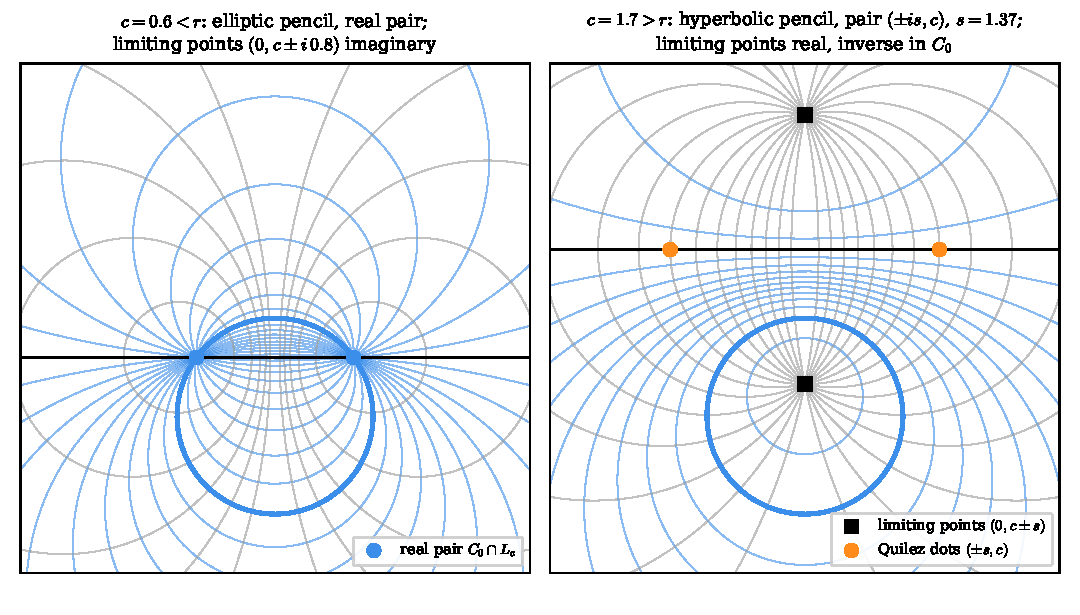
\includegraphics[width=.9\linewidth]{figs/fig5_pencil.pdf}
\caption{The pencil spanned by $K$ and $y=c$ (thin blue) and its orthogonal pencil (grey). Left, $c=0.6$: real common points, conjugate limiting points. Right, $c=1.7$: hidden common points $(\pm is,c)$ and real limiting points $(0,c\pm s)$ (squares); Quilez's dots (orange) are those points rotated by $90^\circ$ about the foot. From \cite{wu}.}\label{fig:pencil}\end{figure}
\begin{proposition}[Limiting points and polarity]\label{prop:polar}\chk{P7.3}
The null points of $V=\mathrm{span}(C,L)$ itself are the \emph{limiting points} of the pencil. For $K$ and $y=c$ they are $(0,c\pm\sqrt{c^2-1})$: real when the common points are hidden ($|c|>1$), and conjugate when they are real. Each limiting point is sent to the other by both $\cdot\star K$ and $\cdot\star L$. The polarity $U\leftrightarrow U^\perp=V$ thus exchanges the common points and the limiting points \cite[Prop.~8]{wu}. Quilez's visible dots $(\pm s,c)$ are the limiting points rotated by $90^\circ$ about the foot $(0,c)$.
\end{proposition}
\begin{proof}
$Q(K+\mu L)=4+4c\mu+\mu^2$, whose roots give the point-circles of centre $(0,c\mp\sqrt{c^2-1})$. The heights multiply to $1$ (inversion in $K$), and they are symmetric about $y=c$ (reflection in $L$). The rest is from Theorem~\ref{thm:common} applied to $V$ instead of $U$.
\end{proof}
\begin{proposition}[Two real forms]\label{prop:sigma1}\chk{P7.4}
$\sigma_1(x,y)=(-\bar x,\bar y)$ is another anti-holomorphic involution preserving circles. Its real circles are $[\alpha:i\beta:\gamma:\delta]$ with $\alpha,\beta,\gamma,\delta\in\R$, on which $Q=-\beta^2+\gamma^2-4\alpha\delta$ has signature $(2,2)$. So $\sigma_1$ defines the real form $PO(2,2)$ of $PO(4,\C)$, next to $\sigma_0$'s $PO(3,1)$. The $\sigma_1$-real points of $K$ are exactly the phantom hyperbola of Prop.~\ref{prop:phantom}. The forms are not conjugate, since their real subspaces have different signatures \cite{wu}.
\end{proposition}
\noindent So the circle and its phantom hyperbola are one complex circle seen through two real structures (Euclidean and Lorentzian). Which common points are visible is a property of the real structure, not of the pair of circles.

\section{Two mirrors}\label{sec:two}
\begin{theorem}\label{thm:two}\chk{T8.1}
Let $M_1,M_2$ be independent mirrors with $\kappa=\kappa(M_1,M_2)\ne1$, $V=\mathrm{span}(M_1,M_2)$ and $T=s_{M_2}s_{M_1}$. Then $T$ is the identity on $U=V^\perp$, preserves $V$, and $T|_V$ has determinant $1$ and trace $4\kappa-2$. So its eigenvalues on $V$ are $\mu^{\pm1}$ with $\mu+\mu^{-1}=4\kappa-2$; writing $\kappa=\cos^2\theta$ ($\theta\in\C$), $\mu=e^{\pm2i\theta}$.
\begin{enumerate}
\item Real lines through a point at angle $\theta$: rotation by $2\theta$, of finite order iff $\theta/\pi\in\mathbb Q$ (Ex.~13: $90^\circ,60^\circ,45^\circ$ give orders $2,3,4$).
\item Parallel lines at distance $\delta$ ($\kappa=1$, excluded above): translation by $2\delta$.
\item Real circles: crossing ($\kappa<1$) gives an elliptic Möbius map; disjoint ($\kappa>1$) a hyperbolic one, with $\mu>0$ real, $\mu\ne1$.
\item Complex angle: for $y=0$ and $y=mx$ with $m=\tan\theta\in\C$, in $u=x+iy$, $v=x-iy$ the map is $u\mapsto\mu u$, $v\mapsto v/\mu$. For $m=i\sqrt3/2$: $\kappa=4$ and $\mu=7\mp4\sqrt3=(2+\sqrt3)^{\mp2}$, a real dilation of $u$ (hyperbolic on the $u$-line) that sends real points to non-real ones.
\end{enumerate}
\end{theorem}
\begin{proof}
$T$ fixes $U\subset M_1^\perp\cap M_2^\perp$. With $P_j=M_jM_j^{\mathsf T}G/Q(M_j)$, $\operatorname{tr}P_j=1$ and $\operatorname{tr}(P_2P_1)=\kappa$, so $\operatorname{tr}T=\operatorname{tr}(I-2P_1-2P_2+4P_2P_1)=4\kappa$, i.e.\ $4\kappa-2$ on $V$; $\det T=1$. Since $\kappa\ne1$, $V$ is non-degenerate and $\C^4=U\oplus V$. (1) and (2) are symbolic computations on point-circles. (3) follows from $\mu+\mu^{-1}=4\kappa-2$: $|\mu|=1$ for $0\le\kappa<1$ and $\mu>0$, $\mu\neq1$ for $\kappa>1$. (4) The rotation identity of (1) is a polynomial identity in $\cos\theta,\sin\theta$ subject to $\cos^2+\sin^2=1$, so it holds for complex $\theta$; in $u,v$ a rotation by $2\theta$ is $u\mapsto e^{2i\theta}u$, $v\mapsto e^{-2i\theta}v$. The case $m=i\sqrt3/2$ was also checked directly.
\end{proof}
\begin{proposition}[Where two mirrors agree]\label{prop:agree}\chk{P8.2}
For $\kappa\ne0,1$ the points $P\in\Qd$ with $P\star M_1=P\star M_2$ are the fixed points of $T$ on $\Qd$: the two common points (null lines of $U$) and the two limiting points (null eigenlines of $T|_V$). Four over $\C$; for real mirrors exactly two of them are real \cite[Thm.~5]{alt}.
\end{proposition}
\begin{proof} $P\star M_1\sim P\star M_2\iff TP\sim P$. Write $P=u+v$. Then $TP=u+Tv$ is proportional to $P$ iff $v=0$, or $u=0$ and $v$ is an eigenvector of $T|_V$. For $\kappa\neq0,1$ the eigenvalues are $\ne\pm1$, so the eigenlines are the two null lines of $V$. \end{proof}

\section{The inverse problem: which mirror swaps two circles?}\label{sec:inverse}
\begin{theorem}\label{thm:inverse}\chk{T9.1}
Let $C,C'$ be independent with $Q(C)Q(C')\neq0$. Rescale $C'$ so that $Q(C')=Q(C)=q$ (possible over $\C$; the two choices differ by sign), and put $p=\ip C{C'}$. A mirror $M$ satisfies $C\star M\sim C'$ iff $M\sim M_\pm:=C\pm C'$ and $Q(M_\pm)=2(q\pm p)\neq0$. Moreover:
\begin{enumerate}
\item $\ip{M_+}{M_-}=0$: the two mirrors are orthogonal; both lie in the pencil of $C,C'$ and hence pass through $C\cap C'$.
\item $Q(M_+)Q(M_-)=4q^2(1-\kappa(C,C'))$. If $C,C'$ are tangent ($\kappa=1$) exactly one candidate is null: it is the point-circle at the contact point, and only one mirror remains.
\item If $C,C'$ are real circles, then $M_\pm$ are real. If they cross ($\kappa<1$), both are real circles or lines (the two bisecting circles); if they are disjoint ($\kappa>1$), one is a real circle and the other has \emph{imaginary radius} (Ex.~16).
\end{enumerate}
\end{theorem}
\begin{proof}
If $\ip CM=0$ then $C\star M=C\not\sim C'$. Otherwise $C\star M=C-kM\sim C'$ with $k\ne0$ forces $M\in\mathrm{span}(C,C')$, say $M\sim C-\lambda C'$. The coefficient of $C$ in $C\star M$ is $1-2\ip CM/Q(M)$, which must vanish: $Q(M)=2\ip CM$, i.e.\ $q-2\lambda p+\lambda^2q=2q-2\lambda p$, i.e.\ $\lambda^2=1$. Conversely, when $\lambda=\pm1$ and $Q(M)\ne0$ the image is a multiple of $C'$. (1) $\ip{C+C'}{C-C'}=Q(C)-Q(C')=0$. (2) The product is $4(q^2-p^2)$. If $\kappa=1$, the null candidate lies in the degenerate pencil and is orthogonal to both $C$ and $C'$ (since $\ip C{C\pm C'}=q\pm p=0$). So it spans the radical $V\cap U$, which is the double common point. (3) For real $C,C'$ with $q>0$ the scaling is real; $Q(M_+)+Q(M_-)=4q>0$ and the product has the sign of $1-\kappa$.
\end{proof}

\section{Relation to Quilez's Short}\label{sec:quilez}
Quilez \cite{IQ} intersects the ray $p=o+\tau d$, $|d|=1$, with $|p|=r$:
\[p=o-d\big(o\cdot d\pm\sqrt{(o\cdot d)^2-|o|^2+r^2}\big),\]
and when the radicand $\Delta$ is negative he draws the real part $o-d(o\cdot d)$ (the foot of the perpendicular) and the points ``real part $\pm$ imaginary part'', placing the imaginary part $\pm\sqrt{|\Delta|}$ \emph{along the line} $d$. The line both rotates and translates, so the trails are tangled. Credit for the construction and the slogan that intersections are always there belongs to him. Video: \url{https://www.youtube.com/shorts/cc-Z_igk4Lo}.

\begin{figure}[t]\centering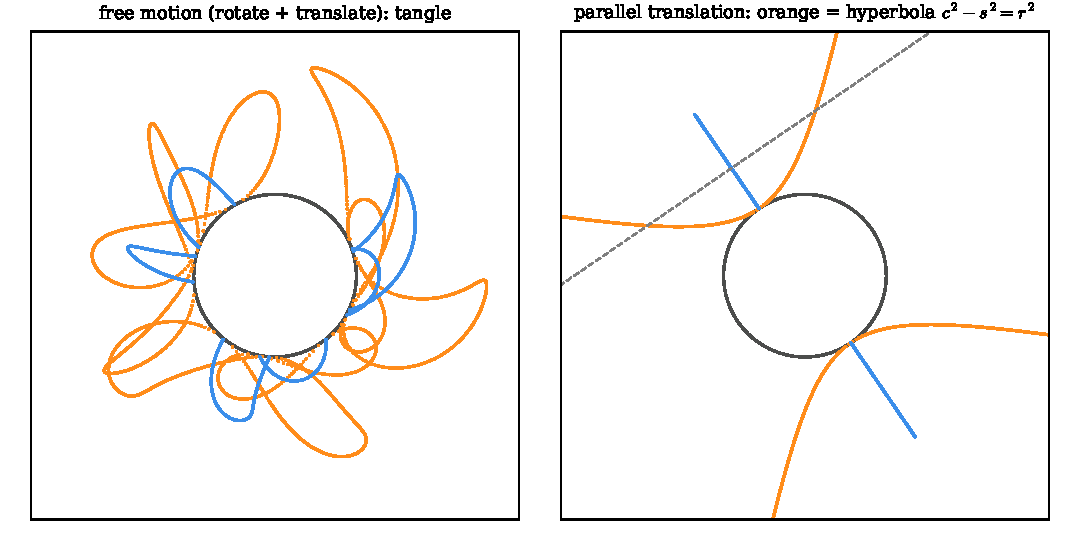
\includegraphics[width=.9\linewidth]{figs/fig2_quilez.pdf}
\caption{Quilez's construction redrawn ($r=1$): blue, the real part; orange, real part $\pm$ imaginary part drawn along the line. Left: free motion. Right: fixed direction, translation only; the orange trail is the hyperbola $c^2-s^2=1$. From \cite{wu}.}\label{fig:quilez}\end{figure}
\emph{Our convention differs in two ways.} (i) We fix the direction and translate only, so the hidden points trace a curve: the hyperbola of Prop.~\ref{prop:phantom}, drawn in $(\Im x,y)$, or in 3D with $\Im t$ as a third axis (Appendix~\ref{app:phantom}). (ii) We do not fold $\Im$ onto the line. Folding is a choice of real slice ($t\mapsto it$), not an operation inside circle space, since $t\mapsto it$ sends circles to hyperbolas (Remark~\ref{rem:Ri}). His folded dots $hn\pm\sqrt{h^2-r^2}\,d$ coincide with our hyperbola. They are also the limiting points of the pencil rotated by $90^\circ$ (Prop.~\ref{prop:polar}, Fig.~\ref{fig:pencil}). In this sense the visible partner of the hidden pair is a genuine Möbius object. Our claims are about the mathematics in his construction; we do not attribute to him any statement made here.

\begin{remark}[The quarter turn is not a mirror]\label{rem:Ri}
The map $R_i:(c,t)\mapsto(c,it)$ in a line frame is not induced by $PO(4,\C)$: it sends the circular points to real points at infinity and $x^2+y^2=r^2$ to $y^2-x^2=r^2$. Inside circle space its role is played by the change of real structure $\sigma_0\to\sigma_1=R_i\sigma_0R_i^{-1}$ (Prop.~\ref{prop:sigma1}). See \cite[Thm.~9]{wu} for this and the stabilizer of $K$ and a parallel pencil (a Klein four-group).
\end{remark}

\appendix
\section{Phantom loci of other curves}\label{app:phantom}
This appendix summarizes \cite{wu}; proofs are given there and checked by \texttt{verify.py} (\textsf{[A.1]} re-checks two numbers).

Let $F\in\R[x,y]$ have degree $k$, $X=\{F=0\}\subset\C^2$, $d$ a real unit direction, $n=d^\perp$, and $f(c,t)=F(cn+td)$. For real $c$ the line $L_c=\{n\cdot p=c\}$ meets $X$ in the roots of $t\mapsto f(c,t)$, a real polynomial, so they are real or come in conjugate pairs. There are $k$ roots with multiplicity unless $d$ is asymptotic ($F_k(d)=0$). The \emph{line-real locus} is $X_d=X\cap(\R\times\C)$, drawn in $(\Re t,c,\Im t)$; its part with $\Im t\ne0$ is the \emph{phantom locus} $\Phi_d(X)$.

\begin{theorem}[Tangency theorem \cite{wu}]
(a) The closure of $\Phi_d(X)$ meets the real plane only at points where $f=f_t=0$, i.e.\ tangencies of $L_c$ with $X_\R$ or singular points. (b) At a smooth tangency of contact order $m$, exactly $m$ smooth branches of $X_d$ meet, at the angles $\pi j/m$ in the $t$-plane. (c) For $m=2$, writing $c=c_0+\tfrac\kappa2(t-t_0)^2+\gamma(t-t_0)^3+\dots$, the phantom branch is $c=c_0-\tfrac\kappa2(\Im t)^2+O(|\Im t|^3)$ with $\Re t-t_0=\tfrac\gamma\kappa(\Im t)^2+O(|\Im t|^3)$: it leaves perpendicular to $X_\R$ with the same curvature, bending the other way.
\end{theorem}
(Here $\kappa$ is a curvature, unrelated to the invariant of §\ref{sec:kappa}.) Examples: for the circle the phantom is the hyperbola $c^2-s^2=r^2$ in the plane $\Re t=0$; for $y=x^2$ it is $c=-s^2$; for $y=x^3-x$ the pairs have $\Re t\ne0$ (at $c=0.6$, $t=-0.6106\pm0.3442i$), so the phantom is not planar. The operator $R_\lambda:(c,t)\mapsto(c,\lambda t)$ has stabilizer $\mu_m$ on a square-free curve, with $m=\gcd$ of the differences of the exponents of $t$ in $f$ \cite[Thm.~5]{wu}. The interactive explorer in the repository draws $X_d$ for several curves.

\section{Verification map}\label{app:ver}
\begin{center}\small\begin{tabular}{ll}\toprule
Statement & Check (log) \\\midrule
Props.~\ref{prop:form}, \ref{prop:segre}, Remark~\ref{rem:IJ} & \textsf{P2.1--P2.3} (\texttt{theory\_verify\_log.txt})\\
Props.~\ref{prop:refl}, \ref{prop:real}; Thm.~\ref{thm:kei} & \textsf{P3.1, P3.2, T3.3}\\
Thm.~\ref{thm:group} & \textsf{T4.1} (numeric decomposition; theorem quoted)\\
Thm.~\ref{thm:common}, Remark~\ref{rem:count} & \textsf{T5.1, E5.2}; all 16 examples (\texttt{examples16\_verify\_log.txt})\\
Prop.~\ref{prop:kappa} & \textsf{P6.1}; random real pairs also in \texttt{verify\_inversive\_log.txt}\\
Props.~\ref{prop:conj}--\ref{prop:sigma1} & \textsf{P7.1--P7.4}; \texttt{verify\_inversive\_log.txt}\\
Thm.~\ref{thm:two}, Prop.~\ref{prop:agree} & \textsf{T8.1, P8.2}; \texttt{alt\_verify\_log.txt}\\
Thm.~\ref{thm:inverse} & \textsf{T9.1}; Ex.~16\\
Appendix~\ref{app:phantom} & \textsf{A.1}; \texttt{verify\_log.txt}\\\bottomrule
\end{tabular}\end{center}

\begin{thebibliography}{99}\small
\bibitem{IQ} I.~Quilez, \emph{Intersections are always there}, YouTube Short, \url{https://www.youtube.com/shorts/cc-Z_igk4Lo}.
\bibitem{wu} C.~Perassi, \emph{Where the hidden intersections live: phantom loci of plane curves in $\C^2$}, companion note \texttt{writeup.pdf}, 2026.
\bibitem{alt} C.~Perassi, \emph{Circles as mirrors: the circle kei, and where two mirrors agree}, companion note \texttt{alt\_quandle\_note.pdf}, 2026.
\bibitem{Art57} E.~Artin, \emph{Geometric Algebra}, Interscience, 1957 (Cartan--Dieudonné theorem, Ch.~III).
\bibitem{Har92} J.~Harris, \emph{Algebraic Geometry: A First Course}, Springer GTM 133, 1992.
\bibitem{Sch79} H.~Schwerdtfeger, \emph{Geometry of Complex Numbers}, Dover, 1979.
\bibitem{Tak43} M.~Takasaki, Abstractions of symmetric functions, \emph{Tohoku Math.\ J.} 49 (1943) 143--207.
\bibitem{Joy82} D.~Joyce, A classifying invariant of knots, the knot quandle, \emph{J.\ Pure Appl.\ Algebra} 23 (1982) 37--65.
\bibitem{Sta15} D.~Stanovsk\'y, The origins of involutory quandles, arXiv:1506.02389.
\end{thebibliography}
\end{document}
